\documentclass[a4paper,11pt]{article}

\usepackage{mlsubmit}
\usepackage{assign-style}
\usepackage{scrextend}

\begin{document}
\setlength\parindent{0pt}

\initmlsubmision{2}{Gurpreet Singh}{150259}

\begin{mlsolution}

    \subsection*{Part 1}
    \begin{addmargin}{1.5em}
        No, name is not a useful attribute in learning a decision tree as splitting on this attribute will have no gain. Non-statistically speaking, there is a lot of variance in the attribute itself, and it will be very inefficient to decide on the basis of name as it can often be a newly observed value.
    \end{addmargin}

    \subsection*{Part 2}
    \begin{addmargin}{1.5em}
        It is not possible to classify the data given perfectly. Looking at data \#4 and \#6, they have the same values for all fields except for `name', however have different target values. Since we shall not use `name' as a decision classifier (as discussed in Part A), therefore we can say that is is not possible to classify the data perfectly.
    \end{addmargin}

    \subsection*{Part 3}
    \begin{addmargin}{1.5em}

        \begin{figure}[h!]\label{tree:q1}
            \center%
            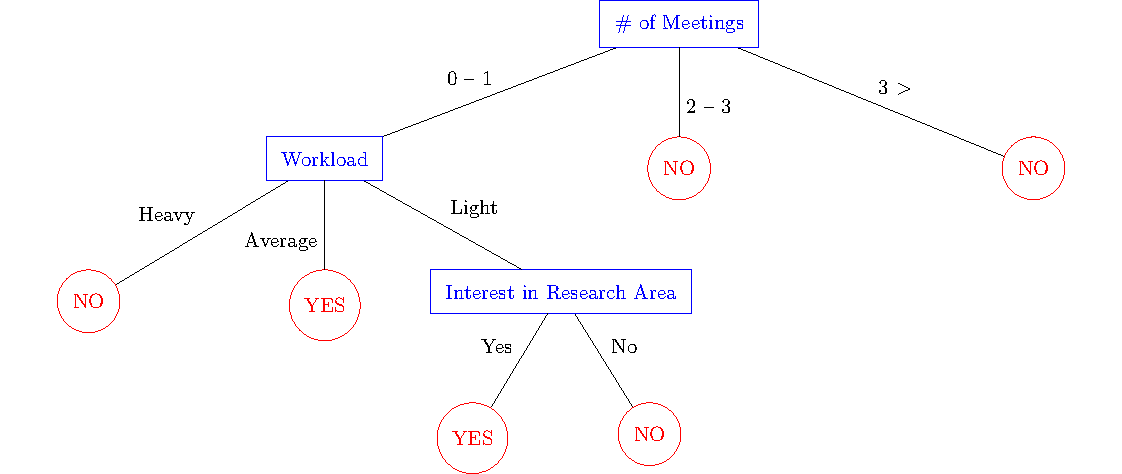
\includegraphics{q1-tree.pdf}
            \caption{ID3 Tree for the given data}
        \end{figure}

        ID3 is a greedy strategy to generate decision trees using Information Gain. The information gain at each level/depth is mentioned below

        \subsubsection{Level 1}
        \begin{addmargin}{1.5em}

            \textbf{Entropy} $S = 0.9183$ \br%

            \textbf{IG:\ Size of Research Group} $ = S - 0.2600 - 0.2667 - 0.3237 = 0.0679$

            \textbf{IG:\ Interest in Research Area} $ = S - 0.2667 - 0.6199 = 0.0317$

            \textbf{IG:\ Workload} $ = S - 0.4000 - 0.2163 - 0.2406 = 0.0614$

            \textbf{IG:\ Number of Meetings} $ = S - 0.6667 = 0.2516$ \br%

            Clearly the attribute \textit{Number of Meetings} provides the most IG, and hence we use this attribute to split at the first level.

        \end{addmargin}

        \subsubsection{Level 2 --- Number of Meetings}
        \begin{addmargin}{1.5em}

            Possible distictions --- `$0 - 1$', `$2 - 3$', `$> 3$' \br%

            Since for `$2 - 3$' and `$> 3$', all labels are `No' (\textbf{i.e.} entropy is $0$), hence we do need to split here, and we add leaf nodes. \br%

            For the samples remaining with value `$0 - 1$' of the attribute \textit{Number of Meetings}, we will further extend the decision tree. \br%

            \textbf{Extropy} $S = 1$ \br%

            \textbf{IG:\ Size of Research Group} $ = S - 0.0000 - 0.4000 - 0.4855 = 0.1145$

            \textbf{IG:\ Interest in Research Area} $ = S - 0.2755 - 0.6897 = 0.0348$

            \textbf{IG:\ Workload} $ = S - 0.0000 - 0.0000 - 0.3610 = 0.6390$
            \br%

            Clearly the attribute \textit{Workload} gives the highest gain, and hence we use this attribute to further construct the decision tree.
            
        \end{addmargin}

        \subsubsection{Level 3 --- Workload}
        \begin{addmargin}{1.5em}

            Possible distinctions --- `Light', `Average', `Heavy' \br%

            Since there is purity in the samples with `Average' and `Heavy' value in the \textit{Workload} attribute (\textit{i.e.} entropy is 0), we do not split further in this case. Therefore we are only left with two samples, which have the value `Light'. \br%

            \textbf{Entropy} $S = 1$ \br%

            \textbf{IG:\ Size of Research Group} $ = S - 1.0000 = 0.0000$

            \textbf{IG:\ Interest in Research Area} $ = S - 0.0000 = 1.0000$ \br%

            Hence we further split using \textit{Interest in Research Area} attribute. Since there is only one sample per distinction, we cannot split further. Hence we have the decision tree showed in Figure~\ref{tree:q1}

        \end{addmargin}

    \end{addmargin}

\end{mlsolution}

\begin{mlsolution}
    
\end{mlsolution}

\begin{mlsolution}

    \begin{qpart}{1}

        We have the optimization problem $(P1)$ as follows

        \begin{align*}
            \label{eq:P1}
            \min_{\vw, \bset{\xi_i}}    &   \norm{\vw}_2^2 + \sum_{i = 1}^{n} \xi_i^2 & (P1) \\
                                        &   s.t. \forall i \in \brac{n} \quad 1 - y^i \dotp{\vw}{\vx^i} \le \xi_i \\
                                        &   \xi_i \ge 0
        \end{align*} \br%

        Now consider an optimization problem $(P2)$, which is similar to the optimization problem given in equation~\ref{eq:P1}, except that we do not have the condition $\xi_i \ge 0$ for any $i \in \brac{n}$. Clearly, the convexity still holds, and hence we will have a solution for $(P2)$. \br%

        Consider this solution to be $\vw_0, \bset{\xi_i^0}$. If we do not have any $k \in \brac{n}$ such that $\xi_k^0 < 0$. Then we can safely claim that the solution for both the optimization problems $(P1)$ and $(P2)$ is the same. Otherwise, we will have at least one $k \in \brac{n}$ such that the condition holds, \textit{i.e.} $\xi_k^0 < 0$. Since this is a solution of the $(P2)$, we can say that this satisfies the condition $1 - y^k \dotp{\vw}{\vx^k} \le \xi_k^0$.

        Now consider the pair $\vw, \bset{\xi_i^1}$ where 

        \begin{align*}
            \xi_i^1 = \begin{cases}
                \xi_i^0     &   if i \ne k \\
                0           &   if i = k
            \end{cases}
        \end{align*} \br%

        Since $0 > \xi_k^0$, we can say that it follows all constraints of $(P2)$ and $0 < \para{\xi_k^0}^2$. For all other $\xi_i^1$, they are the same and hence do not change anything (since all $\xi_i$ are independent). Hence, we can say that $w, \bset{\xi_i^1}$ is a solution of $(P2)$, and $val(P2, \bpara{w, \bset{\xi_i^1}}) < val(P2, \bpara{w, \bset{\xi_i^1}})$. \br%
        
        However, since $w, \bset{\xi_i^0}$ was claimed to be a valid solution, this is not possible. Hence the claim that can exist a $k \in \brac{n}$ such that $\xi_k^0 < 0$ is false. Hence, the solution of $(P2)$ is always the same as that of $(P1)$, which suggests that the second constraint is vacuous.
        
    \end{qpart}

    \begin{qpart}{2}
       
        Since we have already proved that the constraint $\xi_i \ge 0$ is vacuous, we can alter the optimization problem as follows

        \begin{align*}
            \min_{\vw, \bset{\xi_i}}    &   \norm{\vw}_2^2 + \sum_{i = 1}^{n} \xi_i^2 & (P1) \\
                                        &   s.t. \forall i \in \brac{n} \quad 1 - y^i \dotp{\vw}{\vx^i} \le \xi_i
        \end{align*} \br%

        We can convert this problem to an unconstrained optimization problem using Langrange Multipliers.

        \begin{align*}
            & \min_{\vw, \bset{\xi_i}} \max_{\vlambda} \norm{\vw}_2^2 + \sum_{i = 1}^{n} \xi_i^2 + \sum_{i = 1}^{n} \vlambda_i \bpara{1 - y^i \dotp{\vw}{\vx^i} - \xi_i} & (P1)\\
            \label{eq:P1l}
        \end{align*} \br%

        \qnote{Everywhere, $\vlambda \in \R^n$}

    \end{qpart}

    \begin{qpart}{3}

        We can convert the optimization problem $(P1)$ given in equation~\ref{eq:P1l} to a dual problem. Assuming strong duality, we can switch the optimization variables.

        \begin{align*}
            & \max_{\vlambda} \min_{\vw, \bset{\xi_i}} \norm{\vw}_2^2 + \sum_{i = 1}^{n} \xi_i^2 + \sum_{i = 1}^{n} \vlambda_i \bpara{1 - y^i \dotp{\vw}{\vx^i} - \xi_i} & (P1)\\
        \end{align*} \br%

        Now using this, we can first optimize based on the inner optimization (using differentiation). That is, we can partially differentiate w.r.t.\ to $\vw$ and $\bset{\xi_i}$ separately, in order to obtain a dual problem.

        \begin{align*}
            \frac{\partial P1}{\partial \vw}    =& \quad 2\vw - \sum_{i = 1}^{n} \vlambda_i y^i \vx^i = 0 \\
                                                \implies& \quad \pr{\vw} = \frac{1}{2} \sum_{i = 1}^{n} \vlambda_i y^i \vx^i \\
            \\
            \frac{\partial P1}{\partial \xi_k}  =& \quad 2\xi_k - \lamdba_k = 0 \\
                                                \implies& \quad \pr{\xi_k} = \frac{\vlambda_k}{2}
        \end{align*} \br%

        Hence, we can replace these values in the optimization problem, while solving the inner optimization problem.

        \begin{align*}
            & \max_{\vlambda} \quad  \norm{\pr{\vw}}_2^2 + \sum_{i = 1}^{n} \pr{\xi_i}^2 + \sum_{i = 1}^{n} \vlambda_i \bpara{1 - y^i \dotp{\pr{\vw}}{\vx^i} - \pr{\xi_i}} \\
            =& \max_{\vlambda} \quad  \norm{\frac{1}{2} \sum_{i = 1}^{n} \vlambda_i y^i \vx^i}_2^2 + \frac{1}{4} \sum_{i = 1}^{n} \vlambda_i^2 - \sum_{i = 1}^{n} \vlambda_i - \sum_{i = 1}^{n} \vlambda_i y^i \dotp{\frac{1}{2} \sum_{j = 1}^{n} \vlambda_j y^j \vx^j}{\vx^i} - \frac{1}{2} \sum_{i = 1}^{n} \vlambda_i^2 \\
            =& \max_{\vlambda} \quad  \norm{\frac{1}{2} \sum_{i = 1}^{n} \vlambda_i y^i \vx^i}_2^2 - \frac{1}{2} \sum_{i = 1}^{n} \sum_{j = 1}^{n} \vlambda_i \vlambda_j y^i y^j \dotp{\vx^j}{\vx^i} - \frac{1}{4} \sum_{i = 1}^{n} \vlambda_i^2 - \sum_{i = 1}^{n} \vlambda_i
        \end{align*}

        We can expand the first term as

        \begin{align*}
            & \norm{\frac{1}{2} \sum_{i = 1}^{n} \vlambda_i y^i \vx^i}_2^2 = \frac{1}{4} \norm{\sum_{i = 1}^{n} \vlambda_i y^i \vx^i}_2^2 \\
            \implies & \norm{\frac{1}{2} \sum_{i = 1}^{n} \vlambda_i y^i \vx^i}_2^2 = \frac{1}{4} \sum_{i = 1}^{n} \sum_{j = 1}^{n} \vlambda_i \vlambda_j y^i y^j \dotp{\vx^i}{\vx^j}
        \end{align*}

        Replacing back in the original equation

        \begin{align*}
            =& \max_{\vlambda} \quad  - \frac{1}{4} \sum_{i = 1}^{n} \sum_{j = 1}^{n} \vlambda_i \vlambda_j y^i y^j \dotp{\vx^j}{\vx^i} - \frac{1}{4} \sum_{i = 1}^{n} \vlambda_i^2 - \sum_{i = 1}^{n} \vlambda_i \\
        \end{align*}

        We can alter this optimization problem by multiplying with $-4$ and inverting the optimizing condition. Therefore, the final dual optimization problem can be represented as follows

        \begin{align*}
            & \min_{\vlambda \in \R^n} \vlambda^T Q \vlambda + \sum_{i = 1}^{n} \vlambda_i^2 - 4 \vlambda_i & (D1) \\
            \shortintertext{where}
            & Q_{ij} = y^i y^j \dotp{\vx^i}{\vx^j}
        \end{align*}
        
    \end{qpart}

    \begin{qpart}{4}

        Let us state the original dual problem.

        \begin{align*}
            \min_{\valpha \in \brac{0, C}^n} \valpha^T Q \valpha - \sum_{i = 1}^{n} \valpha_i
        \end{align*}

        The main difference that seems to be there between the two objectives is that the dual variable (each value) in the original problem is upper bounded by a constant $C$. \br%
        
        It seems that the dual variable in $(D1)$ has no upper bound, however there is still a tradeoff between the high and low values of our dual variable. Consider $\vlambda > 2$. In this case, the second term will become positive. Hence, we do not want very hight values of $\vlambda$. Looking at the primal problem of the original SVM, we can say that in our case (by similarity of terms), C = 2. Hence we are trying to keep the value of $\lambda$ within the range $\brac{0, C}^n$, however it is a loose bound. \br%
        
        Therefore, the only difference is that in the original SVM problem, we have a strict upper bound on the value of the dual variable, whereas in our case, the upper bound is loose, but still existant.
        
    \end{qpart}

    \begin{qpart}{5}

        \textbf{No}. From our approach, we have proved that $\xi_i < 0$ only increases the value of the objective function while $\xi_i = 0$ is a solution, and hence the lower bound is vacuous, however, this is not the case with the original SVM.\ In the original problem, we are hoping to get negative values of $\xi_i$ which would mean that we are giving weightage to the points which are far from the margin, which is not a correct optimization problem, as it essentials ignores the large margin problem. Hence, in that case, we need to explicitly add the lower bound.

    \end{qpart}

\end{mlsolution}

\begin{mlsolution}
    
\end{mlsolution}

\end{document}
